\documentclass{beamer}
\usepackage[latin1]{inputenc}
\usetheme{Warsaw}
\title[Make a LaTeX presentation using Beamer]{Dynamically kicking balls with a
Nao}
\author{Inge Becht\\ Maarten de Jonge\\ Richard Pronk}
\institute{University of Amsterdam}
\date{June 24, 2012}
\begin{document}

\begin{frame}
\titlepage
\end{frame}

\begin{frame}{Goal of The Project}
    \begin{itemize}
        \item{Making a nao able to kick a ball dynamically}
        \item{Nao plans a kick by making a tradeoff between
             accuracy and stableness}
        \item{Integrating solution  into current Dutch Nao Team code}
    \end{itemize}
\end{frame}

\begin{frame}{What is a Nao?}
    \begin{itemize}
        \item{Humanoid robot}
        \item{Used in the Standard Platform League}
    \end{itemize}
     \begin{figure}[H] 
        \begin{center}
            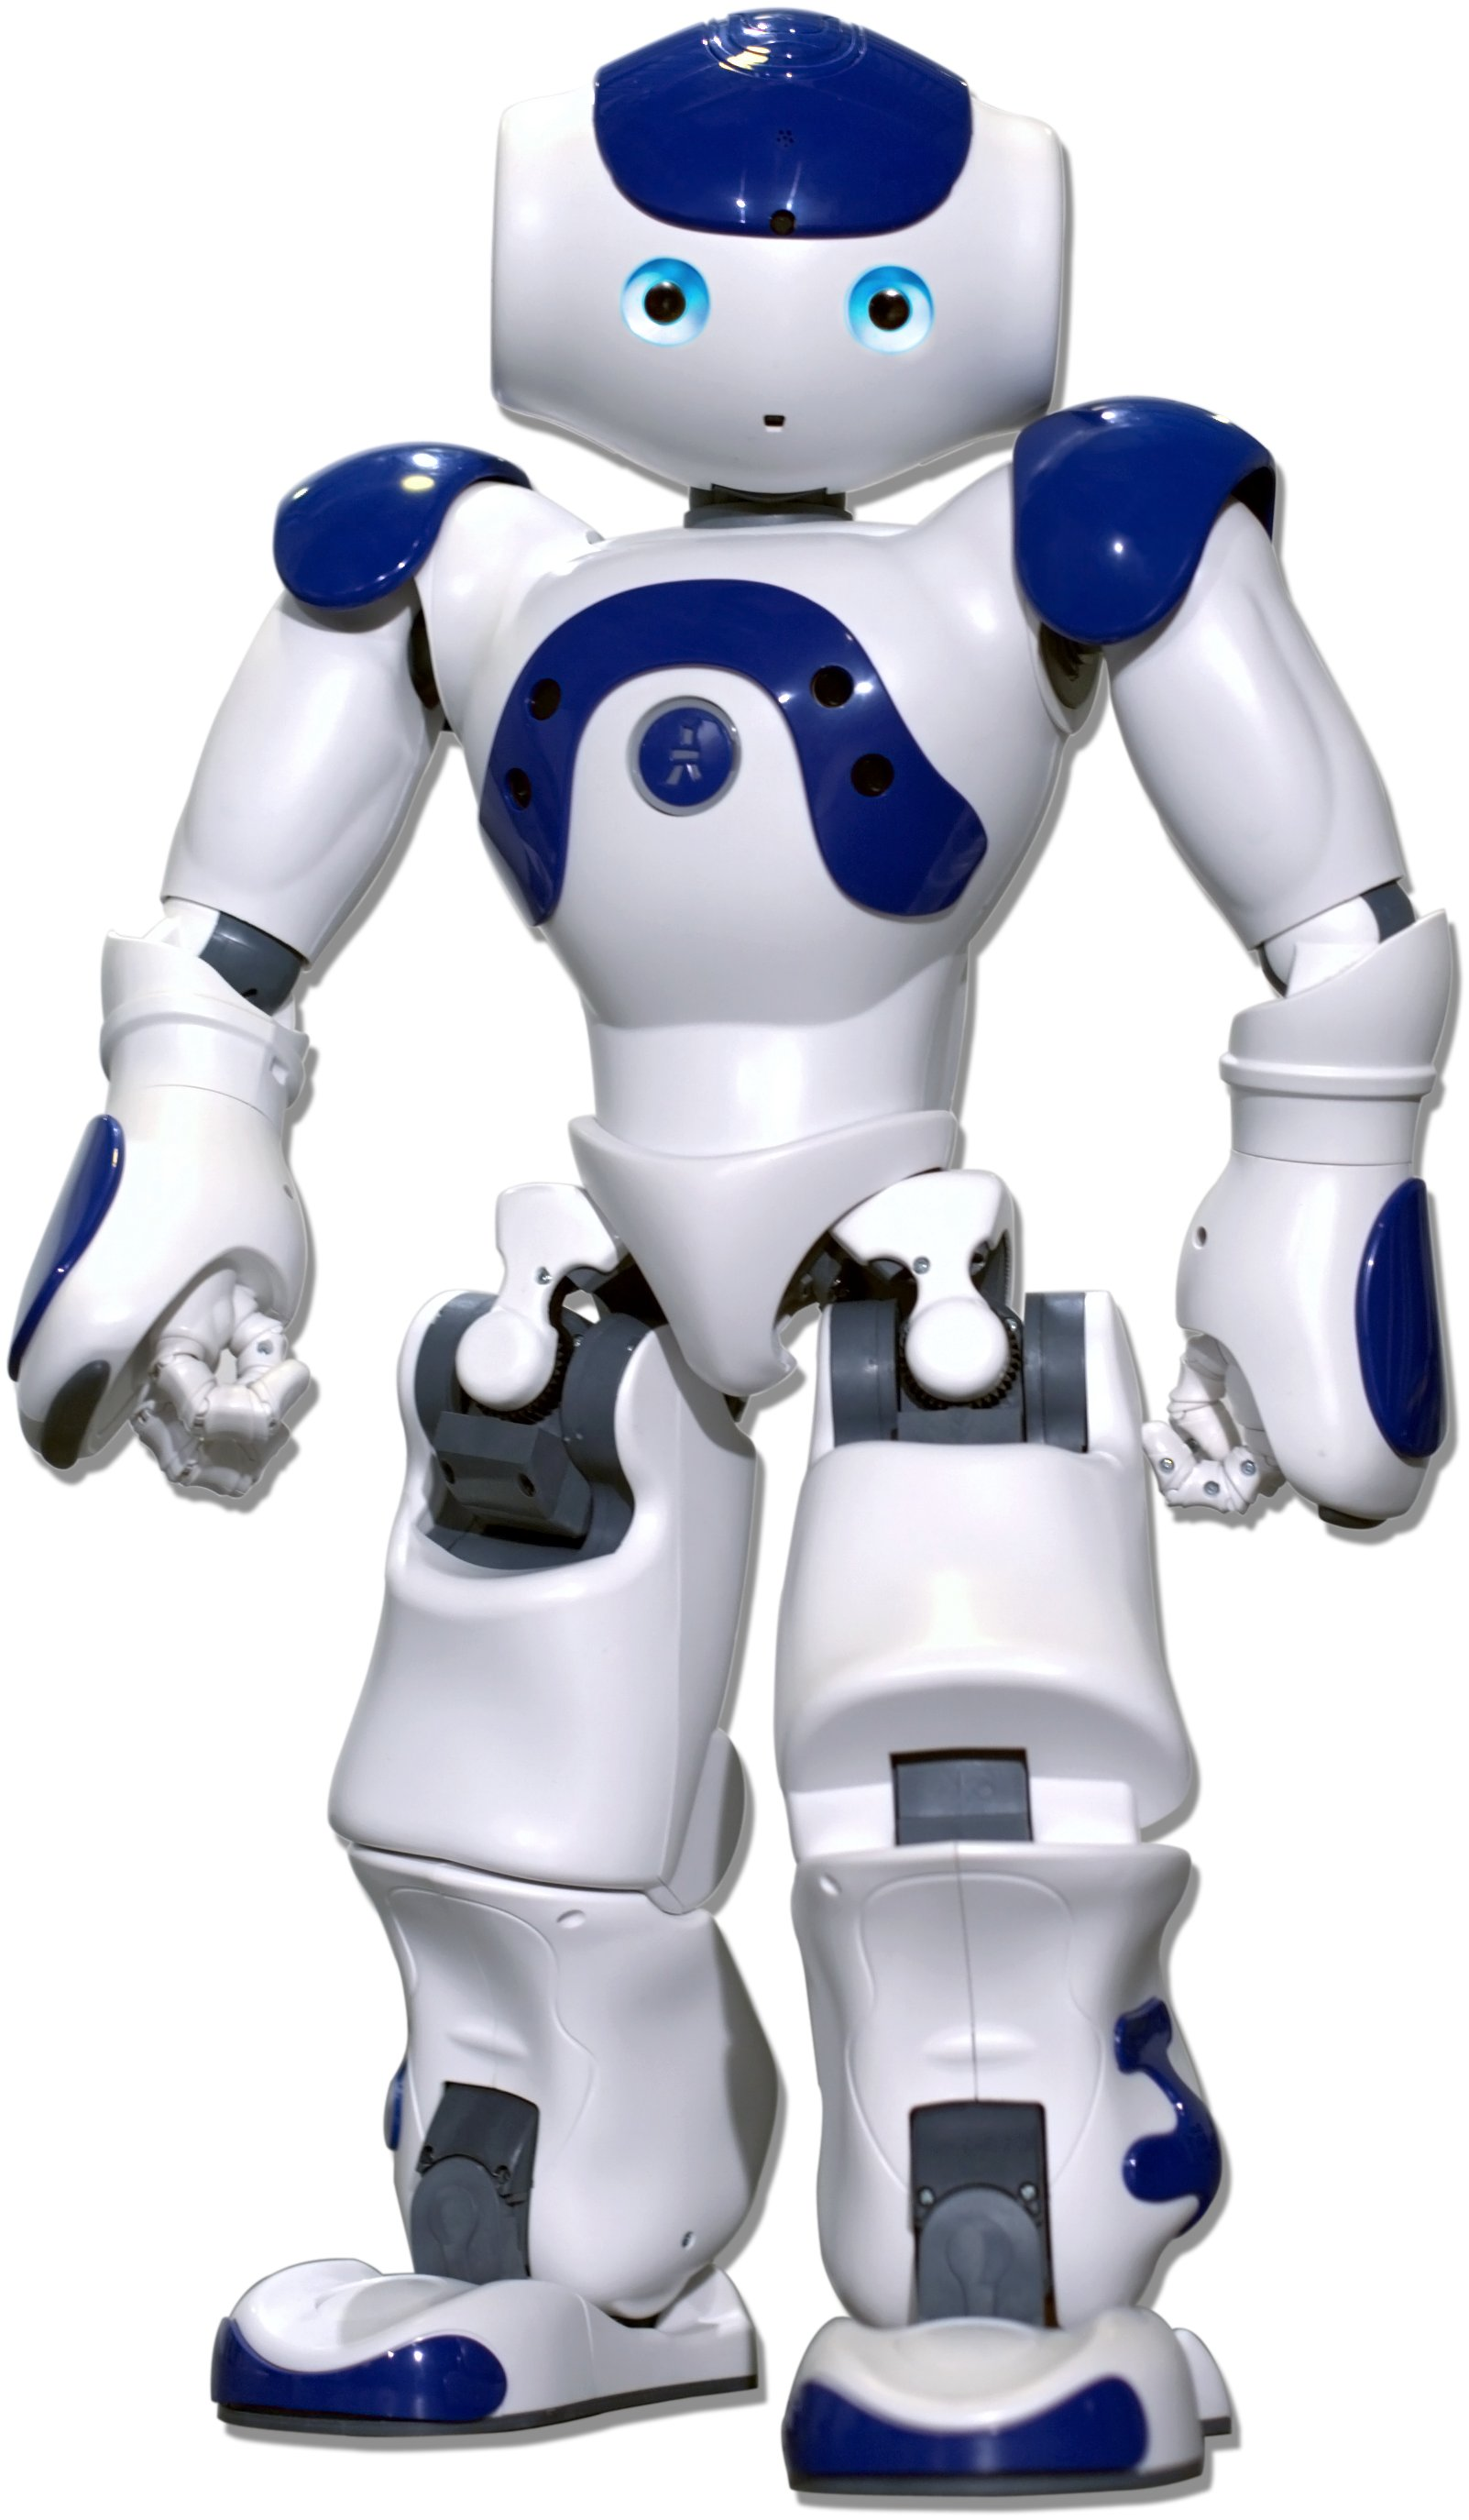
\includegraphics[scale=0.2]{nao.jpg}
            \caption{Nao}
        \end{center}
    \end{figure}  
\end{frame}

\begin{frame}{Why?}
    \begin{itemize}
        \item{Covers same difficulties as walking, but simpler}
        \item{Keyframe motion is brittle}
        \item{More robust  to enviromental factors}
            \begin{itemize}
                \item{Interference by other Naos}
                \item{Compensation for hot joints}
            \end{itemize}
        \item{Will Help the Dutch Nao Team in their next competition}
    \end{itemize}
\end{frame}

\begin{frame}{Possible?}
    \begin{itemize}
        \item{Yes!}
        \item{But quite ambitious}
    \end{itemize}
\end{frame}

\begin{frame}{Data gathered}
    \begin{itemize}
        \item{A lot of papers} 
        \item{All containing a fraction of the whole problem to tackle}
    \end{itemize}
\end{frame}

\begin{frame}{Tasks}
    \begin{itemize}
        \item{Calculating Center of Mass (Currently working on)}
        \item{Calculating the Suport polygon}
        \item{Achieving a inverse kinematica space}
        \item{Evaluating possible kicking motions to be stable enough before
            execution}
    \end{itemize}
\end{frame}

    

\begin{frame}{Introduction}
\end{frame}

\end{document}
